\documentclass[../fractal_dimensions_quasicrystals.tex]{subfiles}
\begin{document}


    	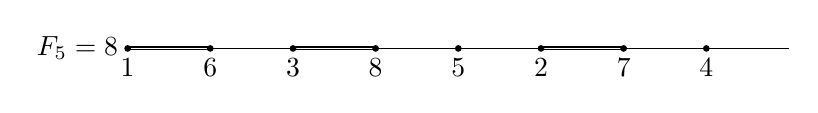
\begin{tikzpicture}[scale=.7]
    		\newcommand{\orig}{-1.5}
    		\newcommand{\trans}{1.5}
    		\newcommand{\vertspac}{-2.}
    	
    		% initial chain
    	
    		% bonds 
        	\draw[-,double] (\orig, 0)  node [left] {$F_{5} = 8$}  -- (\orig+\trans, 0);
			\draw[-] (\orig+\trans,0) -- (\orig+2*\trans,0); % node [midway, above] {$t_s$};
			\draw[-,double] (\orig+2*\trans,0) -- (\orig+3*\trans,0); % node [midway, above] {$t_w$};	
			\draw[-] (\orig+3*\trans,0) -- (\orig+4*\trans,0); % node [midway, above] {$t_s$};
			\draw[-] (\orig+4*\trans,0) -- (\orig+5*\trans,0); % node [midway, above] {$t_w$};
			\draw[-,double] (\orig+5*\trans,0) -- (\orig+6*\trans,0); % node [midway, above] {$t_w$};
			\draw[-] (\orig+6*\trans,0) -- (\orig+7*\trans,0); % node [midway, above] {$t_s$};
			\draw[-] (\orig+7*\trans,0) -- (\orig+8*\trans,0); % node [midway, above] {$t_w$};
    	
    	
    		% sites
		    \filldraw (\orig+0*\trans,0) circle (0.05) node [below] {1};
		    \filldraw (\orig+1*\trans,0) circle (0.05) node [below] {6};
		    \filldraw (\orig+2*\trans,0) circle (0.05) node [below] {3};
		    \filldraw (\orig+3*\trans,0) circle (0.05) node [below] {8};
		    \filldraw (\orig+4*\trans,0) circle (0.05) node [below] {5};
		    \filldraw (\orig+5*\trans,0) circle (0.05) node [below] {2};
		    \filldraw (\orig+6*\trans,0) circle (0.05) node [below] {7};
		    \filldraw (\orig+7*\trans,0) circle (0.05) node [below] {4};
		      
		\end{tikzpicture}

\end{document}